\mansection{quantile}

\begin{mandesc}
  \short{quantile}{sample quantile calculations}
\end{mandesc}

%-- Calling sequence section
\begin{calling_sequence}
\begin{verbatim}
  q = quantile(X, pr)
  q = quantile(X, pr, dim=dimarg, skip_nan=b, meth=num)  
\end{verbatim}
\end{calling_sequence}
%-- Parameters
\begin{parameters}
  \begin{varlist}
    \vname{X}: real vector or matrix, sample values.
    \vname{pr}: real vector with values in $[0,1]$
    \vname{dim=dimarg}: A string chosen among \verb+'M'+, \verb+'m'+, \verb+'*'+,\verb+'full'+, \verb+'FULL'+, \verb+'row'+,
    \verb+'ROW'+, \verb+'col'+, \verb+'COL'+ or an non ambiguous abbreviation or an integer. 
    This argument is optional and if omitted 'full' is assumed.
    \vname{skip_nan=b}: boolean scalar (default is \verb+%f+).
    \vname{meth=num}: a scalar among $\{1,2,3,4,5,6,7,8,9\}$ selecting the quantile algorithm to be used (default is 5).
  \end{varlist}
\end{parameters}

\begin{mandescription}
 Computes for each component $p$ of the vector \verb+pr+ an estimate of the quantile function 
at $p$ from the sample \verb+X+. For a probability distribution associated to a random variable $X$, 
denoting $F(x) = Pr(X \le x)$ its cumulative distribution function (cdf), the quantile 
function is the ``inverse'' of the cdf, precisely:
$$
\mbox{ for } p \in (0,1), \qquad   Q(p) = F^{-1}(p) := inf \{ x \in \R : p \le F(x) \} 
$$
as the cdf is not always continuous and strictly increasing on $\R$ 
(for instance for a discrete random variable).

 For a sample $X=[x_1,x_2,\dots,x_n]$, one can define its empirical cdf:
$$
        F_{empirical}(x) = \frac{\#\{ x_j : x_j \le x \}}{n}
$$ 
and use its inverse (in the meaning seen just before) as quantile estimation (this is
``method 1'' provided by this function). If the sample is sorted then its ``inverse'' is given by :
$$
\mbox{ if } p \in (\frac{i-1}{n},\frac{i}{n}], \quad Q^{(1)}(p) = x_i, \quad i = 1, \dots, n 
$$ 
where we add  $Q^{(1)}(0) = x_1$ to define the function for the whole $[0,1]$ interval. Note that
for all the nine methods, we have always $Q^{(meth)}(0) = x_1$ and $Q^{(meth)}(1) = x_n$. 

In place of using the empirical cdf, one can use different approximations,
(some based on various linear interpolation) and this leads to several methods described here
after. See the following figure corresponding to the sample $X=[1,2,4,7]$.   

$$
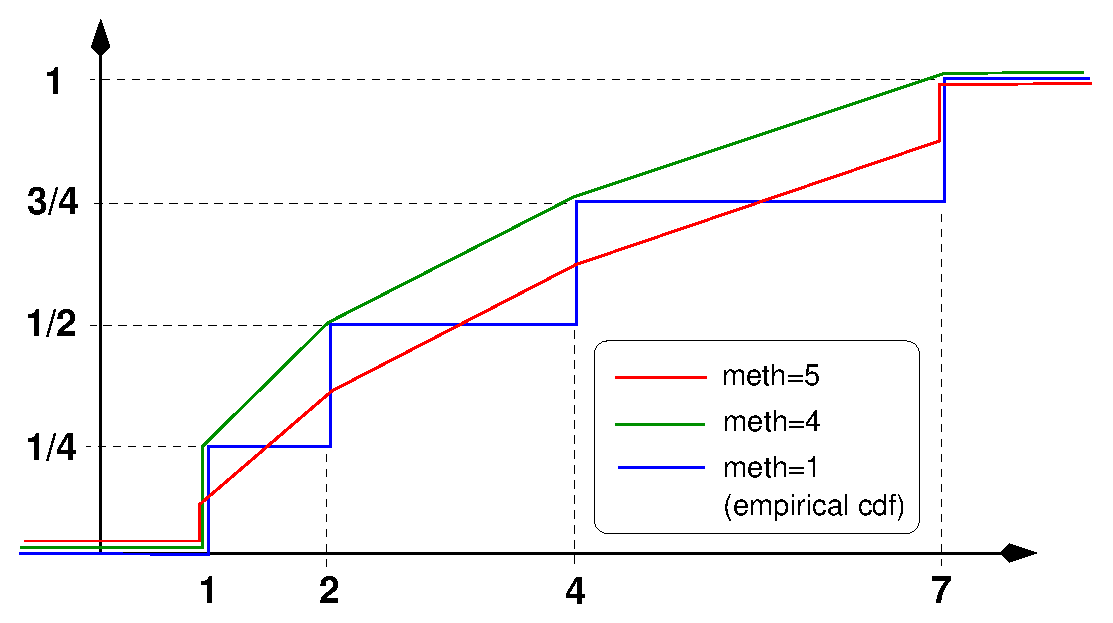
\includegraphics[width=10cm]{fctrep} 
$$



\itemdesc{meth option}

This function (which is modeled from the R and octave quantile functions) provides the 9 methods 
described in Hyndman, R.J.; Fan, Y. (November 1996). "Sample Quantiles in Statistical Packages". 
American Statistician 50 (4): 361-365. We reproduce here the explanations of the R's quantile
help page. 

All the nine sample quantiles are defined as weighted averages of consecutive order statistics
(after sorting the sample vector $X$, $x_1$ is called first order statistic, $x_2$ second order
statistic, $x_j$ $j$th  order statistic, etc...). Sample quantiles of meth $i$ are defined by:
$$
Q^{(i)}(p) = (1 - \gamma) x_j + \gamma x_{j+1}, \quad 1 \le i \le 9, \quad \frac{j-m}{n} \le p < \frac{j-m+1}{n},
$$
n is the sample size. The value of $\gamma$ is a function of $j = floor(np + m)$ and $g = np + m - j$, 
where $m$ is a constant determined by the sample quantile type. 

\begin{description}

\item[Discontinuous sample quantile methods 1, 2, and 3]

For methods 1, 2 and 3, $Q^{(meth)}$ is a discontinuous function of $p$, with $m = 0$ when $i = 1$ 
and $i = 2$, and $m = -1/2$ when $i = 3$.
\begin{itemize}
\item \itemdesc{meth=1} Inverse of empirical distribution function. $\gamma = 0$ if $g = 0$, and $1$ otherwise.

\item \itemdesc{meth=2} Similar to method $1$ but with averaging at discontinuities. $\gamma = 0.5$ if $g = 0$, and $1$ otherwise.

\item \itemdesc{meth=3} SAS definition: nearest even order statistic. $\gamma = 0$ if $g = 0$ and $j$ is even, and $1$ otherwise.
\end{itemize}

\item[~]

\item[Continuous sample quantile methods 4 through 9]

For methods 4 through 9, $Q^{(meth)}$ is a continuous function of $p$, with $\gamma = g$ and $m$ given below. 
The sample quantiles can be obtained equivalently by linear interpolation between the points 
$(p_k,x_k)$ where $x_k$ is the $k$th order statistic. Specific expressions for $p_k$ are given below. 

\begin{itemize}
\item \itemdesc{meth=4} $m=0$, $p_k = k / n$. That is, linear interpolation of the
          empirical cdf.

\item \itemdesc{meth=5} $m=1/2$, $p_k = (k - 0.5) / n$. That is a piecewise linear
          function where the knots are the values midway through the
          steps of the empirical cdf. This is used by matlab's quantile (stat toolbox), and is the default method of octave 's
          quantile, and the default for nsp).

\item \itemdesc{meth=6} $m=p$, $p_k = k / (n + 1)$. This is used by Minitab and by SPSS.

\item \itemdesc{meth=7} $m=1$, $p_k = (k - 1) / (n - 1)$. This is used by S and is the default for R.

\item \itemdesc{meth=8} $m=(p+1)/3$, $p_k = (k - 1/3) / (n + 1/3)$.  The resulting
          quantile estimates are approximately median-unbiased
          regardless of the distribution of $X$.

\item \itemdesc{meth=9} $m = p/4 + 3/8$, $p_k = (k - 3/8) / (n + 1/4)$.  The resulting
          quantile estimates are approximately unbiased for the
          expected order statistics if $X$ is normally distributed.

\end{itemize}
\end{description}

\itemdesc{dim option} 
  The dim argument (default full) gives the dimension to be used for performing the quantile 
calculations (in the following $npr$ will denote the number of components of the vector \verb+pr+):
  \begin{itemize}
    \item 'full' or 0: (default) all the elements of \verb+X+ constitute the sample. If  \verb+X+ is a row
     \verb+q+ is returned as a row vector (with $npr$ components) otherwise \verb+q+ is returned 
     as a column vector (with $npr$ components).
                       
    \item 'row' or 1: each column  of \verb+X+ is a sample ; if  \verb+X+ is an $m \times n$ array
                      so we consider $n$ samples and \verb+q+ is returned as a $npr \times n$ array.
    \item 'col' or 2: each row  of \verb+X+ is a sample ; if  \verb+X+ is an $m \times n$ array
                      so we consider $m$ samples and  \verb+q+ is returned as a $m \times npr$ array.
    \item 'm' (or -2): (for Matlab compatibility) the quantile calculations are done along the first non 
          singleton dimension of the first argument.
  \end{itemize}

\itemdesc{skip\_nan option}
   When this argument is \verb+%t+,  Nan values (which stand for ``missing or not available values'') 
 are not taking into account in the quantile computation.

\end{mandescription}
%--example 
\begin{examples}
\paragraph{example 1} sample quantiles versus exact quantiles for the Gaussian distribution
\begin{Verbatim}
n = 5000;
pr = linspace(0.01,0.99,80)';
X = randn(n,1);  // a sample from N(0,1)
q = quantile(X,pr);
qe = cdfnor("X",zeros(size(pr)),ones(size(pr)),pr,1-pr);
// compare curves
xbasc()
plot2d(pr,[q,qe],style=[2,5],leg="sample quantile@exact quantile",leg_pos="dr")
\end{Verbatim}

\paragraph{example 2} compute quartiles of a sample (and so the inter quartile range (iqr) and the median)
\begin{Verbatim}
n = 500;
X = grand(1,n,"exp",5);
pr = [0.25,0.5,0.75];
q = quantile(X,pr)
iqr = q(3) - q(1)
md = q(2)
// md should be equal to:
median(X)
\end{Verbatim}

\end{examples}

%-- see also
\begin{manseealso}
   \manlink{median}{median}, \manlink{mean}{mean}, \manlink{std}{std}
\end{manseealso}

% -- Authors
\begin{authors}
  Bruno Pincon (designed from the R's quantile help page).
\end{authors}
